\section{Bereitstellung}

Bei der Bereitstellung des gesamten Systems gibt es einen wichtigen Punkt, der beachtet werden muss.
Viele der eingesetzten Services funktionieren als Cluster und benötigen mehrere Server, um ausgeführt zu werden.
Nicht jede Umgebung kann diese Anzahl an Servern bereitstellen.
Daher müssen diese virtualisiert werden.
Dazu wird hier Docker\footnote{https://docker.com} verwendet.
Docker ist eine Laufzeit für Container.
Diese sind ähnlich zu klassischen virtuellen Maschinen, verbrauchen aber weniger Ressourcen.
Ein weiterer Vorteil ist, dass Container für bestimmte Anwendungen gebaut werden.
Ist ein Container einmal gebaut, kann er einfach verteilt und gestartet werden und ist direkt in einem lauffähigen Zustand.
Zum Beispiel gibt es fertige Container, um einen Spark-Master oder -Worker zu starten.
Damit ist der Aufbau eines Spark-Clusters wesentlich einfacher und reproduzierbarer als die Installation in mehreren virtuellen Maschinen.
Zusätzlich gibt es Projekte, wie Kubernetes\footnote{https://kubernetes.io/} oder Docker Swarm\footnote{https://docs.docker.com/engine/swarm/}, die es erlauben Container auf einem verteilten Cluster auszuführen.
Diese werden dann über das Cluster verteilt und über ein virtuelles Netzwerk verbunden.
So wird auch die horizontale Skalierung der verfügbaren Hardware vereinfacht.

Das Ziel ist es, den gesamten Data Lake in Containern bereit zu stellen.
Dabei treten allerdings ein paar Hürden auf, da die verwendeten Rahmenwerke nicht alle auf die Verwendung in Containern ausgelegt sind.
Als erstes muss darauf geachtet werden, dass Container von sich aus keine Persistenz besitzen.
Jenen Daten beziehungsweise Ordnern im Container, die nicht bei einem Neustart verloren gehen dürfen, müssen Volumes\footnote{https://docs.docker.com/storage/volumes/} zugeordnet werden.
Außerdem müssen alle Container im selben Netzwerk sein, damit diese untereinander kommunizieren können.
Da die IP-Adressen, welche die Container in diesen Netzwerken bekommen, nicht außerhalb des Netzwerks erreichbar sind, müssen sowohl das HDFS als auch die SparkSession so konfiguriert werden, dass sie die Host-Namen der Name- und DataNodes verwenden.
Die Host-Namen müssen dann auf die IP-Adresse des Servers aufgelöst werden, auf dem die Container laufen.
Um die Services in den Containern von außen erreichen zu können, müssen die verwendeten Ports freigegeben werden.
Dafür können Ports des Host-Systems zu Ports innerhalb des Containers zugeordnet werden.
Dabei darf ein Host-Port immer nur einmal verwendet werden.

Die Bereitstellung der Services in Docker erfordert den Bau eigener Container.
Als Basis wird das Docker-Image von Python verwendet.
Für jeden Service müssen alle Python-Quell-Dateien kopiert werden.
Bei der Ausführung ist es noch notwendig einen Ordner mit Konfigurationsdateien als Volume in den Container einzubinden.

\subsection{Verwendete Docker Container}

In \cref{fig:docker-datalake} ist ein Beispiel zu sehen, welche Container für ein Data-Lake-System benötigt werden, wie es das Ergebnis dieser Arbeit ist.
Jeder Block repräsentiert einen Container.
Beschrieben werden hier nur die verwendeten Docker-Images und die freigegebenen Ports.
Bei den Ports wird die Notation von Docker benutzt, bei der erst der Host-Port und als zweites der Ziel-Port im Container angegeben wird.
Alle Container liegen in dem gleichen Docker-Netzwerk.
Die grau hinterlegten Gruppen dienen nur der Verdeutlichung der Cluster.
Die Anzahl der Spark-Worker, DataNodes oder Kafka-Broker kann je nach Hardware-Ressourcen angepasst werden.
Alle Container bei denen der Docker-Image-Name mit "`datalake/"' beginnt sind etxra für den Data Lake erstellt.
Das Docker-Image "`datalake/spark"' basiert auf "`bitnami/spark"' und wurde angepasst, die gleiche Python-Version zu verwenden, die auch bei den Services zum Einsatz kommt.

\begin{figure}
    \centering
    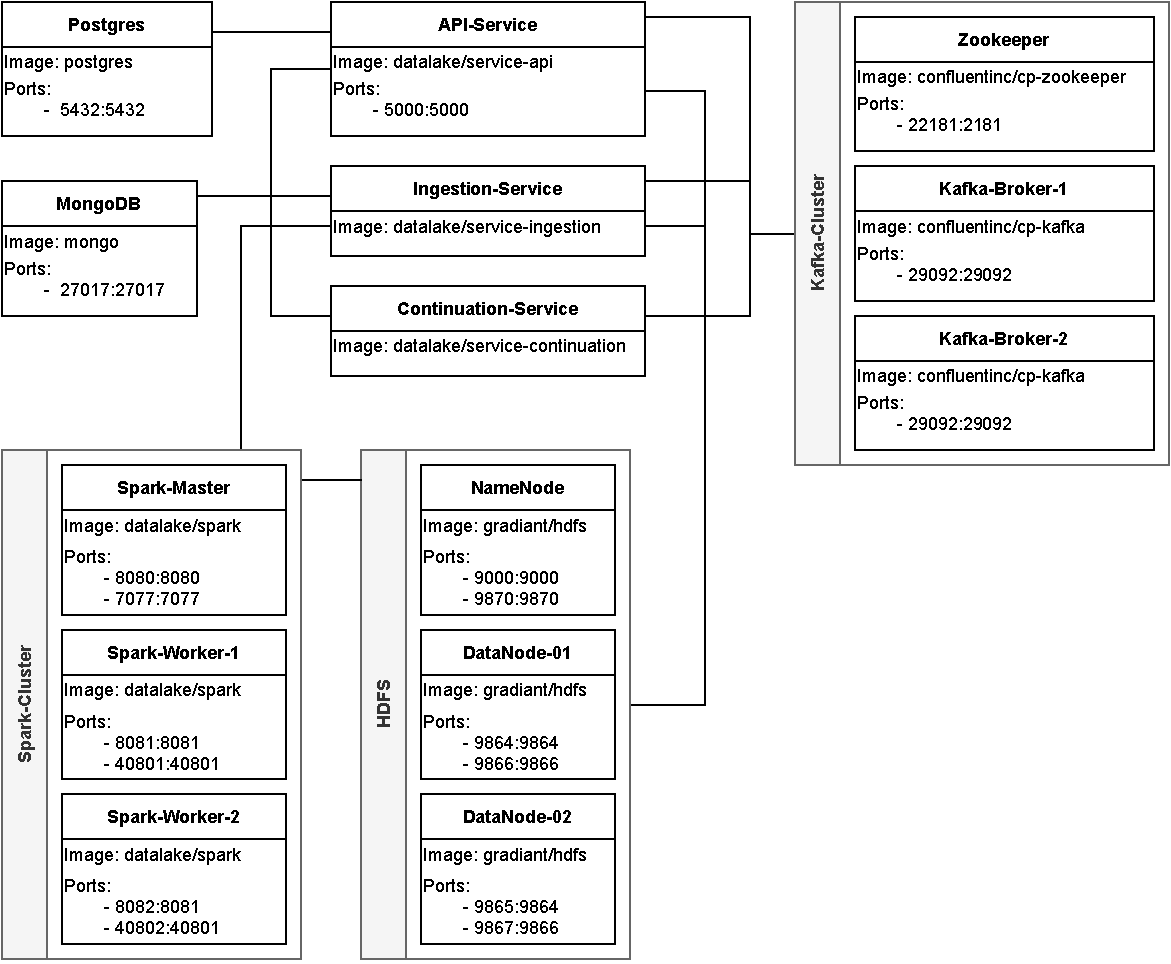
\includegraphics[width=\textwidth]{Grafiken/Umsetzung-Docker-Lake.pdf}
    \caption{Docker-Container für den Data Lake}
    \label{fig:docker-datalake}
\end{figure}
